\chapter{Versuchsdurchführung}
    \section{Arbeitsgerade am Transformator in der Reihenschaltung}  
         
        Zunächst haben wir den Lastwiderstand in Reihe  zum Transformator geschalten \figref{fig:reihenschaltung}. Hier wurde der Lastwiderstand in gewissen Schritten verändert, dabie ändert ich die Spannung $U_{sek}$.
        Im Anschluss wird der Strom $I_{sek}$ errechnet. Die Werte für den Lastwiderstand werden von $12\,\ohm$ auf $22\,\ohm$ um jeweils $2\,\ohm$ erhöht.
        Die Werte wurden in einer Tabelle zusammengetragen \tabref{tab:reihenschaltung}.
        \begin{equation}
            I_{sek}=\frac{U_{sek}}{I_{sek}}
        \end{equation}

        
            \begin{table}[ht!]
                \centering
                \caption{Messwerte zur Reihenschaltung}
                \label{tab:reihenschaltung}
                \begin{tabular}{|c|c|c|}
                    \hline
                    $R_{Last}$ in $\ohm$& $U_{sek}$ in $V$& $I_{sek}$ in $A$\\
                    \hline
                        12 & 18,114 & 1,510\\
                        14 & 18,661 & 1,333\\
                        16 & 19,002 & 1,188\\
                        18 & 19,318 & 1,073\\
                        20 & 19,578 & 0,979\\
                        22 & 19,797 & 0,900\\
                    \hline
                \end{tabular} 
            \end{table}
        Die Auswertung der gemessenen und errechneten Daten wurden mit der Software SciDAVis realisiert \fref{fig:reihenschaltung_aus}. 
        
        \begin{figure}[ht!]
            \centering
            \includegraphics[width=.9\textwidth]{Bilder/u_i_diagramm_reihenschaltung.PNG}
            \caption{Auswertung der Messwerte in der Reihenschaltung}
            \label{fig:reihenschaltung_aus}
        \end{figure}

        Durch die Auswertung mit der linearen Anpassung ergab sich eine Geradengleichung wie folgt.
        \begin{equation}
            U(I)= -2,719\,\ohm\cdot I + 22,244\, V
        \end{equation}
        Dabei ergibt sich eine Leerlaufspannung von
        \begin{equation}
            U_0 = U_{sek}(0\, A) = 22,244\, V 
        \end{equation}
        und ein Kurzschlussstrom von 
        \begin{equation}
            U_{sek}(I_{sek})\overset{!}{=} 0\,\Rightarrow\, I_k = \frac{22,244\, V}{2,719\,\ohm}= 8,181\, A
        \end{equation}
        Die Steigung der Geradengleichung gibt hier den durchschnittlichen Innenwiderstand. Dieser beträgt $2,719\,\ohm$.

    \section{Arbeitsgerade am Transformator in der Parallelschaltung} 
        Im Anschluss wurde das gleiche mit der Parallelschaltung durchgeführt\figref{fig:parallelschaltung}. Hier war der Wertebereich des Lastwiderstands zwischen $4\,\ohm$ und $14\,\ohm$. Auch diese Werte wurden in einer Tabelle zusammengetragen \tabref{tab:parallelschaltung}
        \begin{table}[ht!]
            \centering
            \caption{Messwerte zur Parallelschaltung}
            \label{tab:parallelschaltung}
            \begin{tabular}{|c|c|c|}
                \hline
                $R_{Last}$ in $\ohm$& $U_{sek}$ in $V$& $I_{sek}$ in $A$\\
                \hline
                    4 & 9,502 & 2,375\\
                    6 & 9,991 & 1,665\\
                    8 & 10,256 & 1,282\\
                    10 & 10,421 & 1,042\\
                    12 & 10,534 & 0,878\\
                    14 & 10,617 & 0,758\\
                \hline
            \end{tabular} 
        \end{table}
        Die Werte wurden ebenfalls mit der Software SciDAVis ausgewertet \fref{fig:parallelschaltung_aus}


        \begin{figure}[ht!]
            \centering
            \includegraphics[width=.9\textwidth]{Bilder/u_i_diagramm_parallelschaltung.PNG}
            \caption{Auswertung der Messwerte in der Parallelschaltung}
            \label{fig:parallelschaltung_aus}
        \end{figure}

    
        Auch hier wurde mit Hilfe der linearen Anpassung die Geradengleichung aufgestellt, diese wie folgt lautet.
        \begin{equation}
            U(I)= -0,690\,\ohm\cdot I + 11,140\, V
        \end{equation}
        Dabei ergibt sich eine Leerlaufspannung von
        \begin{equation}
            U_0 = U_{sek}(0\, A) = 11,140\, V 
        \end{equation}
        und ein Kurzschlussstrom von 
        \begin{equation}
            U_{sek}(I_{sek})\overset{!}{=} 0\,\Rightarrow\, I_k = \frac{11,140\, V}{0,690\,\ohm}= 16,145\, A
        \end{equation}
        Auch hier gibt die Steigung der Geradengleichung den durchschnittlichen Innenwiderstand an. Dieser beträgt $0,690\,\ohm$.
    \newpage
    
    \section{Brückengleichrichter mit Glättungskondensator}
        In der nächsten Aufgabe wurde der Brückengleichrichter \figref{fig:gleichrichter} in LTSpice mit einem nicht geladenen Konensator simuliert.
        Die wurde ermöglicht in dem man die Simulation in den ersten $100\, ms$ betrachtet \fref{fig:unaufgeladenner_kondensator}

        \begin{figure}[ht!]
            \centering
            \includegraphics[width=.9\textwidth]{Bilder/unaufgeladenner_kondensator.png}
            \caption{Simulationskurven mit nicht geladenen Kondensator}
            \label{fig:unaufgeladenner_kondensator}
        \end{figure}

        Um ein eingeschwungenes Schaltbild zu erzeugen wird die Simulation mit einem Offset von $0,9\, s$ für $100\, ms$ gestartet.

        \begin{figure}[ht!]
            \centering
            \includegraphics[width=.9\textwidth]{Bilder/aufgeladenner_kondensator.png}
            \caption{Simulationskurven mit eladenen Kondensator}
            \label{fig:aufgeladenner_kondensator}
        \end{figure}

    \newpage
    \section{Wirkungsgrad}
        Für die Ermittlung des Wirkungsgrades wird die Schaltung aus der vorherigen Aufgabe angepasst \fref{fig:schaltbild_wirkungsgrad}.
        Die Änderung die vorgenommen wird ist beim Laststrom. Dieser wird auf $1\, A$ geändert.\par
        \begin{figure}[ht!]
            \centering
            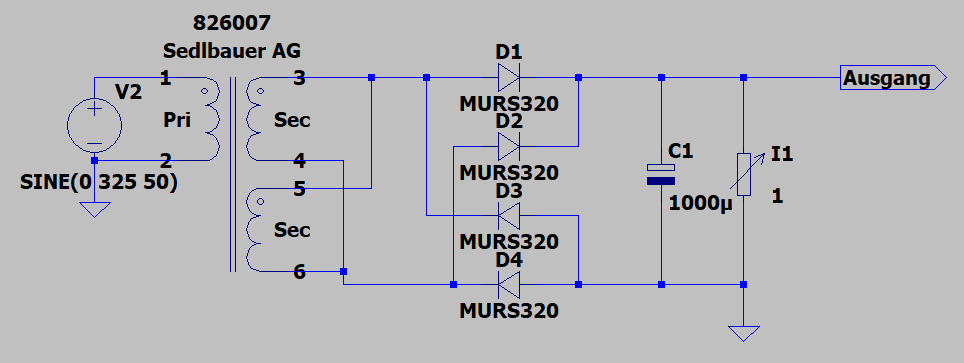
\includegraphics[width=.9\textwidth]{Bilder/wirkungsgrad.png}
            \caption{Schaltbild für die Simulation und Auswertung des Wirkungsgrades}
            \label{fig:schaltbild_wirkungsgrad}
        \end{figure}

        Die Leistung der einzelnen Bauteile wird aus LTSpice abgelesen. 
        \begin{center}
            \begin{tabular}{l r}
                \hline
                Bauteile & Leistung \\
                \hline
                $\overset{-}{P}_{Prim}$& $10,436\, W$ \\
                $\overset{-}{P}_{Last}$ & $-16,852\, W$ \\
                $\overset{-}{P}_{D_1}=\overset{-}{P}_{D_4}$ & $389,87\, mW$\\
                $\overset{-}{P}_{D_2}=\overset{-}{P}_{D_3}$ & $392,92\, mW$\\
                $\overset{-}{P}_{C_1}$ & $-36,759\, mW$\\
                $\overset{-}{P}_{sek}$ & $4,883\, W$\\
                \hline
            \end{tabular} 
        \end{center}

        Setzt man nun die mittlere Leistung des Lastwiderstand $\overset{-}{P}_{Last}$ und der Spannungsquelle $\overset{-}{P}_{Prim}$ in die Gleichung für die berechnung des Wirkungsgrads, so erhält man 

        \begin{equation}
            \mu=\frac{P_{Nutz}}{P_{Aufwand}}= \frac{\overset{-}{P}_{Last}}{\overset{-}{P}_{Prim}}= \frac{10,436\, W}{16,852\, W}= 0,619 = 61,9\%
        \end{equation}

        Wenn man alle Einzelleistungen aufsummiert, exklusive der Primärspulenleistung, ergibt sich: 
        \begin{equation}
            \overset{-}{P}_{Last}+2\cdot\overset{-}{P}_{D_1}+2\cdot\overset{-}{P}_{D_2}+\overset{-}{P}_{C_1}+\overset{-}{P}_{sek}= \overset{-}{P}_{alle}
        \end{equation}

        \begin{equation}
            10,436\, W+2\cdot 389,87\, mW+2\cdot 392,92\, mW + 36,759\, mW + 4,883\, W = 16,139\, W 
        \end{equation}
        Das Ergebnis ist ungefähr der Primärleistung und die logische Konsequenz des addierens aller Teilleistungen.


